\documentclass{article}
\usepackage[section]{placeins}
\usepackage{graphicx, wrapfig, amsmath, amssymb, physics, hyperref}
\hypersetup{
    colorlinks=true,
    linkcolor=blue,
    filecolor=magenta,      
    urlcolor=cyan,
    }

\author{Yaghoub Shahmari}
\title{Report - Problem Set No 6}
\date{\today}
\graphicspath{ {../Figs/} }

\begin{document}
    \maketitle
    \section*{Problem 1}
    \textbf{Basic description:}

    In this problem, we're going to collect samples of the sum of a specific number of particles.
    According to the central limit theorem, this distribution must be gaussian.
    As we can see the results approved the theorem.

    \textbf{The results:}

    \begin{figure}[!htb]
        \centering
        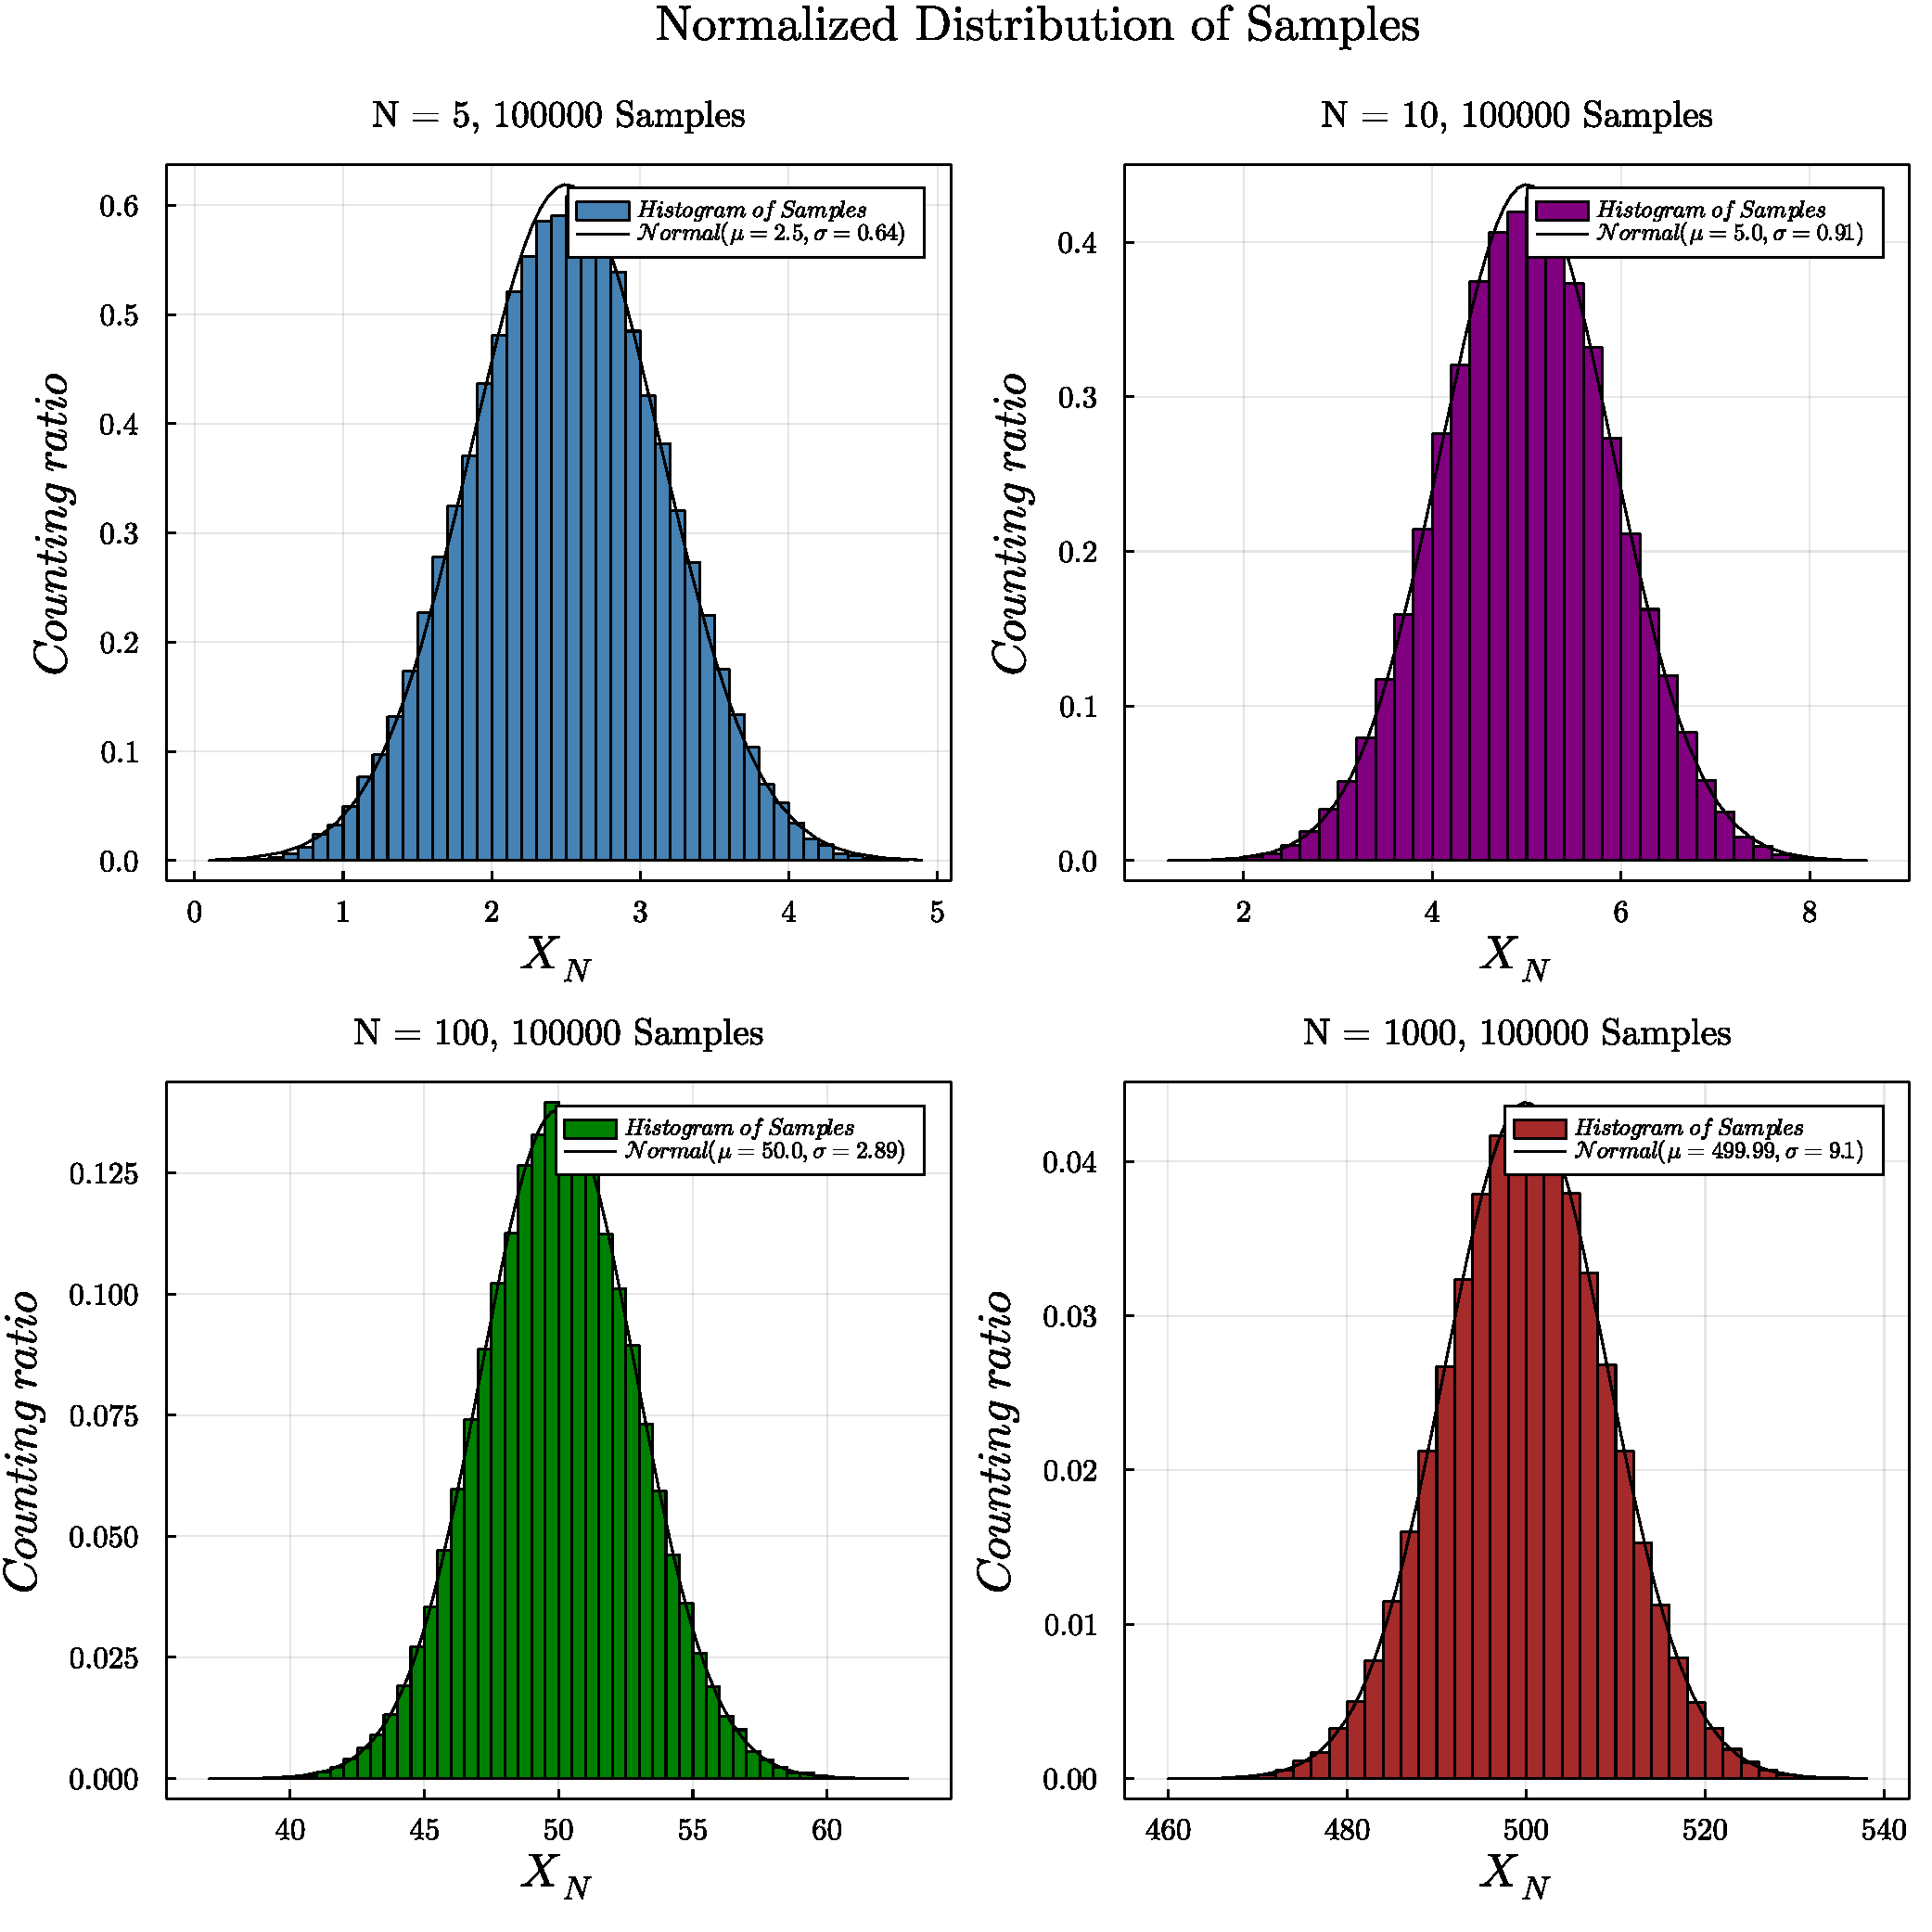
\includegraphics[scale = 0.25]{/Q1/Q1-Hist}
        \label{fig:1.1}
        \caption{Histogram of the distribution of the samples.}
    \end{figure}

    \pagebreak

    \section*{Problem 2}
    \textbf{Basic description:}

    In this problem, we're going to convert a uniform distribution to a gaussian.
    So we continue the book solution. We have x1 and x2 samples.
    To find y1 and y2 (that are from the gaussian distribution) we continue this solution:

    \begin{gather*}
        f_{(x)} dx=g_{(y)} dy \Rightarrow \int f_{(x)} dx = \int g_{(y)} dy\\
        \Rightarrow x = \int g_{(y)} dy = G_{(y)}\\
        \Rightarrow x = {G^{-1}}_{(x)}\\
        g(y) = \frac{e^{-\frac{y^2}{2\sigma^2}}}{\sqrt{2\pi\sigma^2}}
    \end{gather*}

    We know G(y) can't be expressed as we want,
    so we use the box-muller solution to get what we want:

    \begin{gather*}
        g_{(y_1,y_2)dy_1 dy_2 = g_{(y_1)}g_{(y_1)}} = \frac{e^{-\frac{{y_1}^2 + {y_2}^2}{2\sigma^2}}}{2\pi\sigma^2} dy_1 dy_2
    \end{gather*}

    We transform into polar coordinates:

    \begin{gather*}
        y_1 = \rho \sin_{\theta}, \ y_2 = \rho \cos_{\theta}\\
        \Rightarrow g_{(y_1,y_2)}dy_1 dy_2 = g_{(\rho,\theta)}\rho \theta = \frac{e^{-\frac{\rho^2}{2\sigma^2}}}{2\pi\sigma^2}\rho d{\rho}d{\theta}\\
        \Rightarrow {g_1}_{(\rho)} = \frac{e^{-\frac{\rho^2}{2\sigma^2}}}{\sigma^2}\rho d{\rho}d{\theta},\ {g_2}_{(\theta)} = \frac{1}{2\pi} \\
        \Rightarrow {G_1}_{(\rho)} = 1 - e^{-\frac{\rho^2}{2\sigma^2}} ,\ {g_2}_{(\theta)} = \frac{\theta}{2\pi}\\
        \Rightarrow \ \rho = \sigma \sqrt{2ln(\frac{1}{1-x_1})},\ \theta = 2\pi x_2
    \end{gather*}

    So we use the following formula to transform uniform distribution to gaussian distribution.

    \pagebreak

    I also built a function to create a uniform distribution. So, initially I call my uniform distribution creator function and transform the distribution to the Gaussian distribution.

    \textbf{The results:}

    \begin{figure}[!htb]
        \centering
        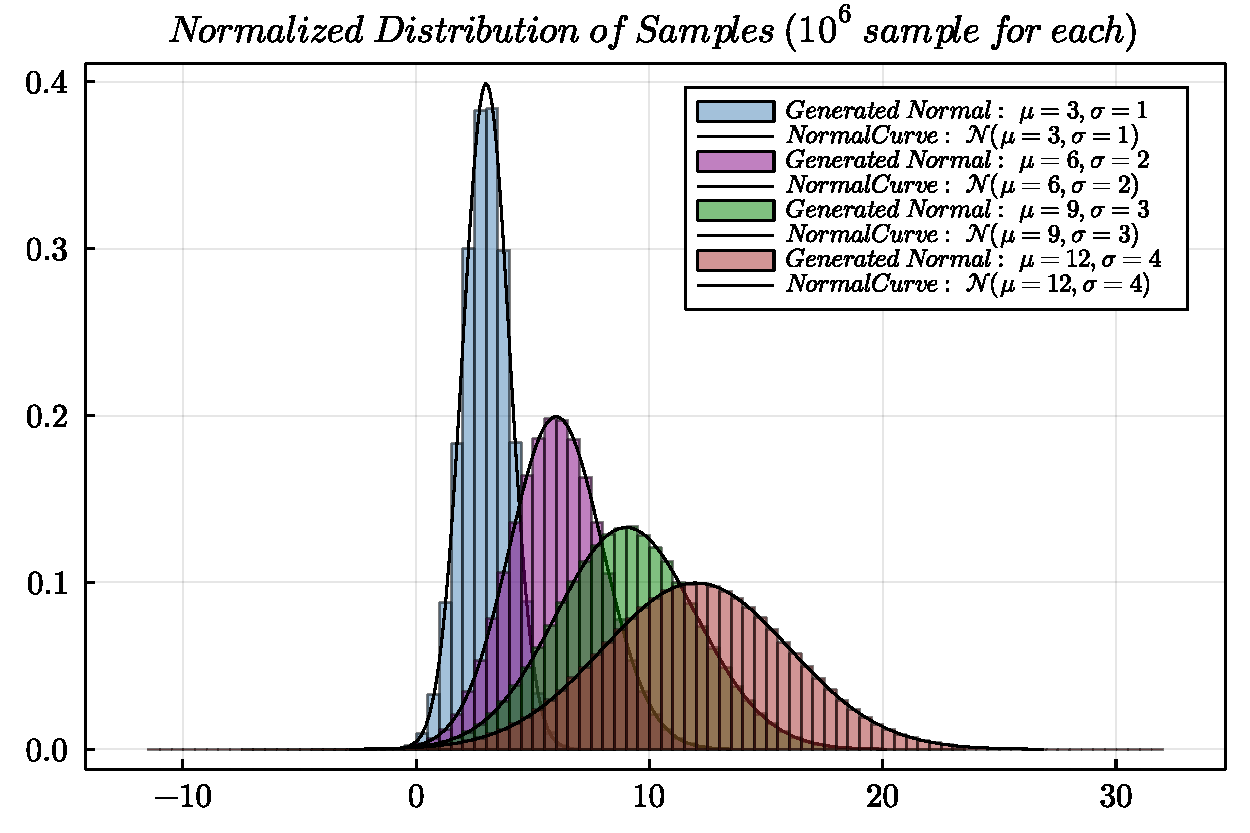
\includegraphics[scale = 0.5]{/Q2/Q2-Hist}
        \label{fig:2.1}
        \caption{Histogram of the distribution of the samples.}
    \end{figure}

    \centering
    \textbf{The whole data I gathered is in \href{https://github.com/shahmari/ComputationalPhysics-Fall2021/tree/main/ProblemSet6/Data}{this link}}

    Thanks for watching :)
\end{document}